\chapter{PENGENALAN ANTARMUKA DAN MENAMBAHKAN DATA SIG PADA APLIKASI QGIS}

Pada Bab ini kita akan mengenal bagian-bagian dasar yang biasa digunakan untuk membuat peta menggunakan QGIS 2.14, menambahkan data, dan mengeksplor data menggunakan \textit{tools-tools} yang tersedia.

\begin{enumerate}[A.]

\item \textbf{Pengenalan Antarmuka QGIS 2.14 Essen}

Bagian-bagian dari antarmuka QGIS ini seperti terlihat pada gambar \ref{fig:bagianui}.

\begin{figure}
  \centering
  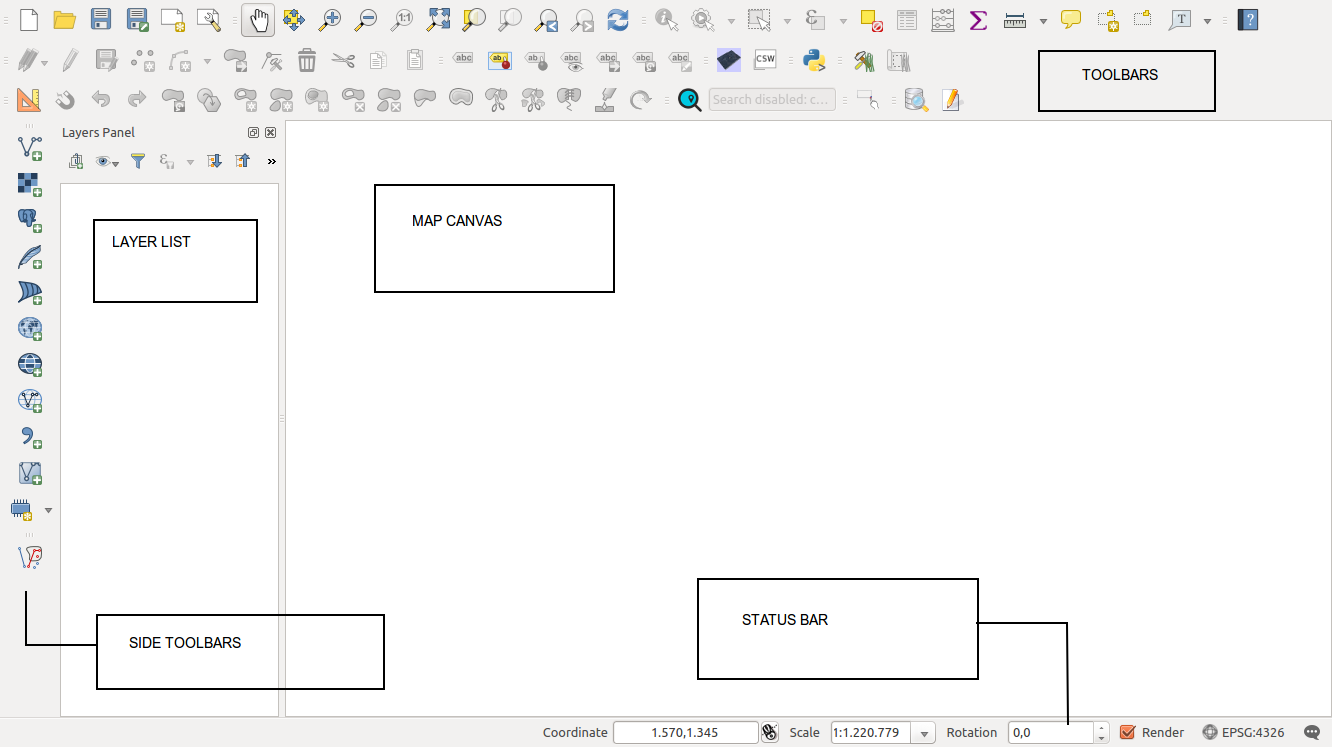
\includegraphics[width=1\textwidth]{./resources/004-bagian-qgis}
  \caption{Bagian Antarmuka QGIS}
  \label{fig:bagianui}
\end{figure}

\begin{itemize}

\item \textbf{Map Canvas}

Merupakan tempat menampilkan proyek / peta yang sedang dijalankan.

\item \textbf{Layer List}

Memuat daftar \textit{layer-layer} yang digunakan dalam proyek. Urutan \textit{layer} yang ditampilkan pada \textit{map canvas} berdasarkan urutan dari atas ke bawah pada \textit{layer list}-nya.

\item \textbf{Menu}

Bagian \textit{menu} ini tidak terlihat di gambar karena konfigurasi tampilan \textit{menu} menempel pada \textit{menu bar desktop}. \textit{Menu} ini berisi sekumpulan perintah teks untuk melakukan tugas-tugas tertentu.

\item \textbf{Toolbar dan Side Tooldbar}

Bagian ini berisi sekumpulan perintah berbasis tombol / ikon untuk melakukan tugas-tugas tertentu. \textit{Tools} dikelompokan dalam grup-grup \textit{toolbar} seperti \textit{File Toolbar}, \textit{Digitizing Toolbar}, \textit{Managed Layers Toolbar}, dan lainnya.

\item \textbf{Status Bar}

\textit{Status bar} memuat koordinat berdasarkan lokasi kursor / pointer, skala, dan sistem koordinat proyek pada \textit{map canvas}.

\end{itemize}

\item \textbf{Menambahkan Data}

\item \textbf{Mengeksplor Data}

\end{enumerate}